\section{Brief Bios of the Principals}

\parbox{5.0in}{
\begin{wrapfigure}{l}{2in - .75\columnsep} %{3.8in}{2.0in} %{0.45\textwidth}
  % \centering
    \vspace{-\intextsep}
    \hspace*{-.15\columnsep}\includegraphics[scale=0.3]{fig/Faguado.jpg}
\end{wrapfigure}
\textbf{Fernando Aguado} is an Associate Professor at the University
of Vigo. He was the principal investigator (PI) of the Xatcobeo
cubesat, the first Galician satellitor swapping
them with those fully charged. e and the first Spanish
cubesat. He was also the PI of HUMSAT-D and sector B of Serpens (both
developed within the Basic Space Technology Initiative of UN with the
support of ESA) and the LUME-1 \smle. He has coordinated the design,
manufacturing and integration of various Cubesats for maritime and
airplane tracking applications as well as for inter-vehicle
communications. 
\\
\textbf{email: }\emph{faguado@tsc.uvigo.es} \\
\textbf{Web: }\url{https://bit.ly/3avJlwX}\\
}

\vspace*{3cm}
\parbox{6.5in}{
\begin{wrapfigure}{r}{3.8in - .75\columnsep} %{3.8in}
  \vspace{-\intextsep}
    \hspace*{-.35\columnsep}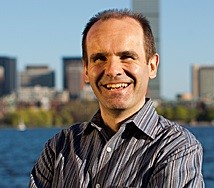
\includegraphics[scale=0.3]{fig/Pierre.jpg}
\end{wrapfigure}
\textbf{Pierre Lermusiaux} is Professor of Mechanical Engineering and
Ocean Science and Engineering at MIT, and, since July 2018, Associate
Department Head for Research and Operations in Mechanical
Engineering. He has made outstanding contributions in data
assimilation, as well as in ocean modeling and uncertainty
predictions. His research thrusts include understanding and modeling
complex physical and interdisciplinary oceanic dynamics and processes
while utilizing new mathematical models and computational methods for
ocean predictions and dynamical diagnostics for data assimilation
and data-model comparisons.
\\
\textbf{email: }\emph{pierrel@mit.edu}\\
\textbf{Web:}\url{http://web.mit.edu/pierrel/www/} 
}

\parbox{6.3in}{
\begin{wrapfigure}{r}{3.6in - .75\columnsep} %{3.8in}{0.45\textwidth}
  % \centering
    \vspace{-\intextsep}
    \hspace*{-.35\columnsep}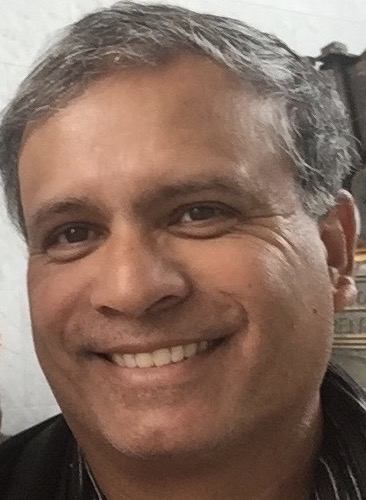
\includegraphics[scale=0.4]{fig/KRajan.jpg}
\end{wrapfigure}
\textbf{Kanna Rajan} is a Fellow at SIFT LLC and holds a visiting
faculty appointment at \univ in autonomous systems. At \inst his
software was responsible for the command/control of the 1999 New
Millennium Deep Space 1, 65 Million miles from Earth and the 2003 Mars
Exploration Rovers mission on the Red Planet. In 2005 he moved to \mba
to build the only AI group in marine robotics and to focus on using
AI-based machine intelligence for marine robotics and biological
oceanography. His publications have been in highly ranked
peer-reviewed publications while his field work includes scientific
oceanographic cruises in the Pacific and the Atlantic.
\\
\textbf{email: }\emph{Kanna.Rajan@sift.net}\\
\textbf{Web:}\url{https://kanna.rajan.systems} }

\vspace*{3cm}
\parbox{5.5in}{
\begin{wrapfigure}{l}{2.0in - .75\columnsep} %{3.8in}{0.45\textwidth}{0.45\textwidth}
  % \centering
  \vspace{-\intextsep}
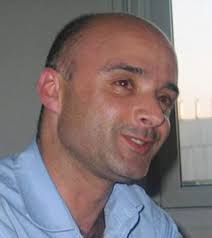
\includegraphics[scale=0.06]{fig/JBS.jpg}
\end{wrapfigure}
\textbf{Jo\~ao Sousa} is a Professor at the Faculty of Engineering,
Univ. of Porto, Portugal and the head of the Underwater Systems and
Technology Laboratory (\lse). The lab has pioneered the design,
construction and deployment of networked underwater, surface and air
vehicles for applications in ocean sciences and defense and is at the
vanguard of operations of coordinated aerial, surface and underwater
vehicles. The lab designed the award-winning Light Autonomous
Underwater Vehicle and the \ls open source software for networked
vehicle systems, and has been key in organizing large scale
experiments, including the annual Rapid Environmental Picture (\rpe)
organized jointly with the Portuguese Navy since 2010. He has
participated and led numerous engineering and scientific oceanographic
cruises.
\\
\textbf{email: }\emph{jtasso@fe.up.pt}\\
\textbf{Web: }\url{https://lsts.pt/team/joao-sousa}}
% {https://lsts.pt/member/jo%C3%A3o-sousa}

\center{
% \vspace*{0.5cm}
\parbox{5.5in}{
\begin{wrapfigure}{l}{2.0in - .75\columnsep} %{3.8in}{0.45\textwidth}{0.45\textwidth}{0.45\textwidth}
 % \centering
   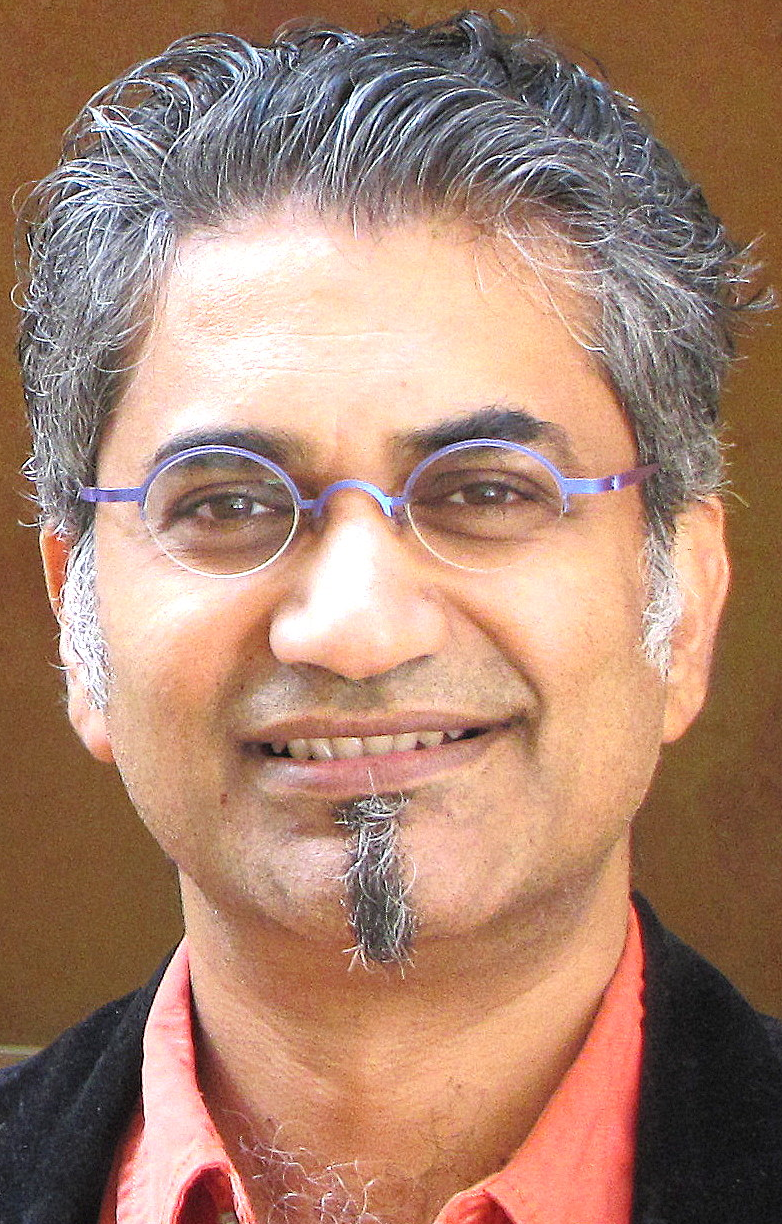
\includegraphics[scale=0.15]{fig/ASub.png}
\end{wrapfigure}

\textbf{Ajit Subramaniam} is a Lamont Research Professor at the
Lamont-Doherty Earth Observatory (\ldeoe) of Columbia University, New
York.  He is an oceanographer who uses knowledge of remote sensing,
ocean optics, phytoplankton physiology, biological and physical
oceanography and geographical information systems to better understand
how the marine ecosystem functions and can be managed.  He has worked
for National Oceanic and Atmospheric Administration (NOAA), %  and held
% appointments at the Univ. of Maryland and the Univ. of Southern
% California 
 prior to moving to \ldeo in 2004. He has served as the Program
Director for the Marine Microbiology Initiative at the Gordon and
Betty Moore Foundation and a program manager in the Biological
Oceanography Program at the U.S. National Science Foundation (NSF). He
has participated in oceanographic cruises in all parts of the world.
\\
\textbf{email: }\emph{ajit@ldeo.columbia.edu} \\
\textbf{Web: }\url{https://www.ldeo.columbia.edu/~ajit/}
}

\vspace*{3cm}
\parbox{6.5in}{
\begin{wrapfigure}{r}{3.8in - .75\columnsep} %{0.45\textwidth}
 % \centering
  \vspace{-\intextsep}
    \hspace*{-.35\columnsep}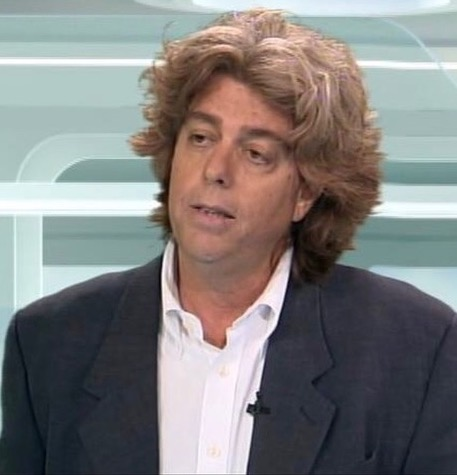
\includegraphics[scale=0.25]{fig/JTintore.jpeg}
\end{wrapfigure}

\textbf{Joaqu\'{i}n Tintor\'{e}} is Professor of Physical Oceanography
and Director of the Spanish Large-Scale Marine Infrastructure SOCIB
(Balearic Islands Coastal Ocean Observing and Forecasting System) that
he proposed and designed in 2006. His present scientific interest is
in understanding ocean state and variability, from episodic events to
climate variability from the coast to the open ocean while
implementing new multi-platform and integrated ocean observing and
forecasting systems.
\\
\textbf{email: }\emph{jtintore@socib.es} \\
\textbf{Web:
}\url{http://www.socib.eu/?seccion=textes&id_textotextes=director} }
}
